\documentclass[12pt]{article}
\usepackage[utf8]{inputenc}
\usepackage{graphicx} % Allows you to insert figures
\usepackage{amsmath} % Allows you to do equations
\usepackage{fancyhdr} % Formats the header
\usepackage{geometry} % Formats the paper size, orientation, and margins
\linespread{1.25} % about 1.5 spacing in Word
\setlength{\parindent}{0pt} % no paragraph indents
\setlength{\parskip}{1em} % paragraphs separated by one line
\usepackage[style=authoryear-ibid,backend=biber,maxbibnames=99,maxcitenames=2,uniquelist=false,isbn=false,url=true,eprint=false,doi=true,giveninits=true,uniquename=init]{biblatex} % Allows you to do citations - does Harvard style and compatible with Zotero
\urlstyle{same} % makes a nicer URL and DOI font 
\AtEveryBibitem{
    \clearfield{urlyear}
    \clearfield{urlmonth}
} % removes access date
\AtEveryBibitem{\clearfield{month}} % removes months in bibliography
\AtEveryCitekey{\clearfield{month}} % removes months in citations
\renewbibmacro{in:}{} % Removes the "In" before journal names

\renewbibmacro*{editorstrg}{%from biblatex.def
  \printtext[editortype]{%
    \iffieldundef{editortype}
      {\ifboolexpr{
         test {\ifnumgreater{\value{editor}}{1}}
         or
         test {\ifandothers{editor}}
       }
         {\bibcpstring{editors}}
         {\bibcpstring{editor}}}
      {\ifbibxstring{\thefield{editortype}}
         {\ifboolexpr{
            test {\ifnumgreater{\value{editor}}{1}}
            or
            test {\ifandothers{editor}}
          }
            {\bibcpstring{\thefield{editortype}s}}%changed
            {\bibcpstring{\thefield{editortype}}}}%changed
         {\thefield{editortype}}}}}

\renewbibmacro*{byeditor+others}{%from biblatex.def
  \ifnameundef{editor}
    {}
    {\printnames[byeditor]{editor}%
     \addspace%added
     \mkbibparens{\usebibmacro{editorstrg}}%added
     \clearname{editor}%
     \newunit}%
  \usebibmacro{byeditorx}%
  \usebibmacro{bytranslator+others}}
  % The commands above from lines 20-49 change the way editors are displayed in books
\AtEveryBibitem{%
  \clearlist{language}%
} % removes language from bibliography
\citetrackerfalse 
% Removes ibids (ibidems)
\DeclareNameAlias{sortname}{family-given} % Ensures the names of the authors after the first author are in the correct order in the bibliography
\renewcommand*{\revsdnamepunct}{} % Corrects punctuation for authors with just a first initial
\addbibresource{Example.bib} % Tells LaTeX where the citations are coming from. This is imported from Zotero
\usepackage[format=plain,
            font=times new roman]{caption} % Italicizes figure captions
\usepackage[english]{babel}
\usepackage{csquotes}
\renewcommand*{\nameyeardelim}{\addcomma\space} % Adds comma in in-text citations
\renewcommand{\headrulewidth}{0pt}
\geometry{letterpaper, portrait, margin=1in}
\setlength{\headheight}{29.49998pt}

\newcommand\titleofdoc{CS51 Final Project Report} %%%%% Put your document title in this argument
\newcommand\GroupName{Jared Hu Ni} %%%%% Put your group name here. If you are the only member of the group, just put your name

\begin{document}
\begin{titlepage}
   \begin{center}
        \vspace*{4cm} % Adjust spacings to ensure the title page is generally filled with text

        \Huge{\titleofdoc} 

        \vspace{0.5cm}
            
        \vspace{3 cm}
        \Large{\GroupName}
       
        \vspace{0.25cm}
       
        \vspace{3 cm}
        \Large{May 4, 2022}
        
        \vspace{0.25 cm}
        \Large{CS51: Abstraction and Design in Computation}
       

       \vfill
    \end{center}
\end{titlepage}

\setcounter{page}{1}
\pagestyle{fancy}
\fancyhf{}
\rhead{\thepage}
\lhead{\titleofdoc}

\section{Introduction}

In the CS51 final project, I was given the opportunity to implement an interpreter for the MiniML language, a functional subset of the OCaml language that has both concrete and abstract syntax and is capable of evaluating basic functional operations. It has truly been a fun project to work on: from implementing the helper functions in expr.ml to the various evaluators, I have had moments of excitement and periods of excitement, but I had never felt bored. Though I have learned a lot through each and every stage of this conceptually challenging yet rewarding project, I feel especially compelled to share with you my personal extensions to MiniML language, as I have completed for stage 8 of the project. 

My first extension was the added support for unit, float, and string types. The original MiniML source code only included support for a limited number of atomic types, including integer, variables, booleans, and complex types such as functions, binary and unary operations. in a real programming language, there are much more atomic types that the programmer can work with to perform various tasks. So, I had decided to make it my goal to extend upon the basics and include some of the most fundamental atomic types that define a modern programming language into MiniML. Using OCaml's algebraic data types, I had successfully implemented unit, float, and string types, extended the unary and binary operations to accommodate for these new types (such as string concatenation and float operations), and went through rounds of intensive testing to make sure the interpreter performs the way that I have intended on these new types. 

My second extension was implementing the lexical evaluator for the interpreter. The project only required us to complete the substitution and the dynamic evaluators, but neither of them fully models the way that an actual OCaml interpreter works. The OCaml language, in its elegance, utilizes the lazy nature of the dynamic environment, yet outputs results that are identical to the substitution model because it has lexical environment semantics. Implementing and testing the lexical evaluator in MiniML has given me a better grasp of how the lexical environment functions, and it has been, by far, one of the most engaging topics I had the opportunity to learn this semester. 


\pagebreak
\section{Implementation of Atomic Types}

In this section, I will explain in detail how I added support for the float, string, and unit types in MiniML. On the surface, the new types are simply extended as additional algebraic data types in type expr, and the operations performed on them are additional algebraic data types in type binop and type unop. In type expr of the expr.ml file, I added Float, String, Unit, and FunUnit (for functions that take in unit); in type binop, I added Concat (for concatenating two strings), FloatPlus, FloatMinus, and FloatTimes (for operating on floats). In type unop, I added FloatNegate (to negate a float). To make the interpreter recognize and understand these new types, we must modify the MiniML Lexical Analyzer (miniml\_lex.mll) and MiniML Parser (miniml\_parse.mly) files. 


In the lexical analyzer, keywords of the language are defined in the keyword\_table, and symbols are defined in the sym\_table. the sym\_table is where I matched the concrete syntax of new operators to their parser-recognizable abstract data type counterparts (notice how these are capitalized versions of the algebraic data types given in expr.ml). These capitalized types correspond to the tokens defined in the parser, where the grammar rules for using and operating on these data types are mapped to their corresponding algebraic data types, outputting the abstract syntax defined using these grammar rules when declaring or performing an operation. For example, FLOAT carries a float type, so its corresponding abstract syntax would be Float \$1 (where \$1 is a placeholder signifying the place that the data is located in the grammar expression). exp FLOATPLUS exp corresponds to Binop(FloatPlus, \$1, \$3), where \$1 is the first exp (expression) and \$3 is the second exp. 

In the lexical analyzer, a new rule token must be added for each of the new atomic types (except unit) to recognize and process the syntactic pattern and structure using OCaml's regular expressions (regex), so that the new type can be recognized by the interpreter. For example, in the given source code, an integer is recognized as anything composed of digit numbers 0 through 9 and has a length of at least 1. Its rule token recognizes the said pattern and convert the string to an int type. The finished product, recognized as an INT, can then be used to evaluate expressions given the grammar rules defined in the parser. Extending upon the example, I developed the rule tokens to process and recognize floats and strings; using regex, a float is recognized as repeated digits like that of the integer before and after the symbol ".", a decimal dot. A string is the repetition of any characters except double quotes and double-backslash within a pair of double quotes. I then had to process string to remove all double-quotes in the rule token, so the double quotes disappear in the event of string concatenation, and they reappear in the concrete and abstract syntax if printed. 

After the lexical analyzer and parser are able to accommodate the new atomic types and their operations, I extended the case match in every function of expr.ml and the evaluation.ml to include these new types and the behaviors of using their binary and unary operations. This process is very similar to implementing the functional behavior of the other atomic data types and operations given in the source code, so I will not bore you with the details. 

\section{Demonstration of the Atomic Types}

The following demonstrations are the behaviors performed by my MiniML interpreter, which I have modified to display the interpretation of all three evaluators that I have implemented: eval\_s for substitution, eval\_d for dynamic environment, and eval\_l for lexical environment.

Here are some mathematical operations that utilize the float type. In the picture below, float 4.2 and float 42. are added (+.), multiplied (*.), subtracted (-.), and negated (~-.) in the MiniML interpreter in using the three evaluators implemented. 
\begin{center}
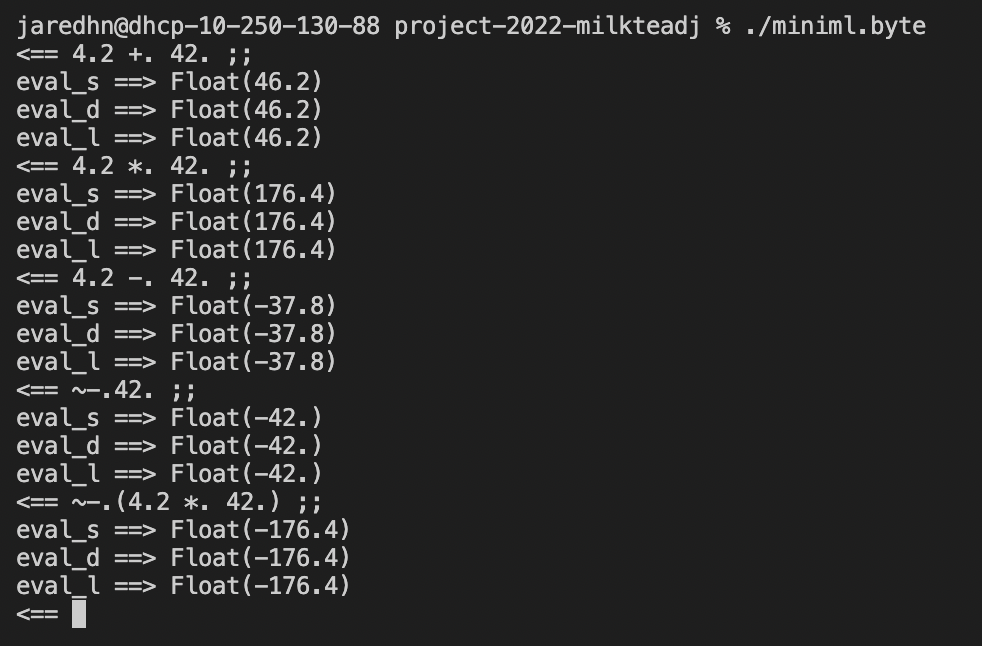
\includegraphics[width=15cm]{floats.png}\\
Float operations in the MiniML interpreter
\end{center}

Here are some string concatenation operations. In the first example, a function called f takes in the string "42 is" as the argument, and the argument is concatenated to " 42" and outputs the string "42 is 42". In the second example, three sub-strings are concatenated to construct the sentence, "abstraction is its own reward". 
\begin{center}
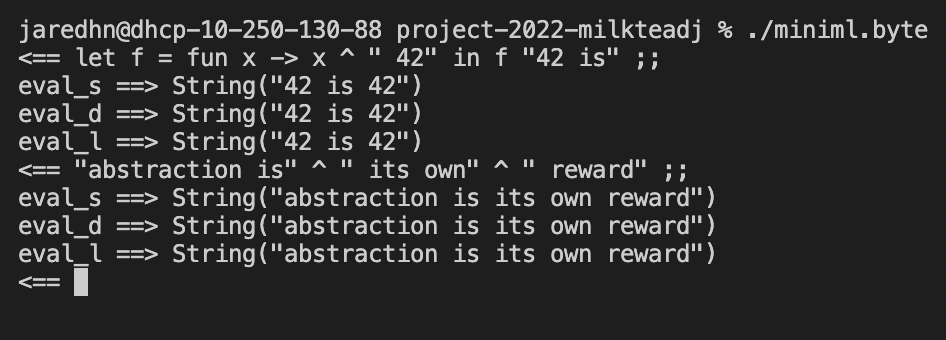
\includegraphics[width=15cm]{string.png}\\
String operations in the MiniML interpreter
\end{center}

Here are operations using unit type. the unit type can be printed on its own, or it can be used as a function argument in FunUnit functions that take in a unit as its argument. 
\begin{center}
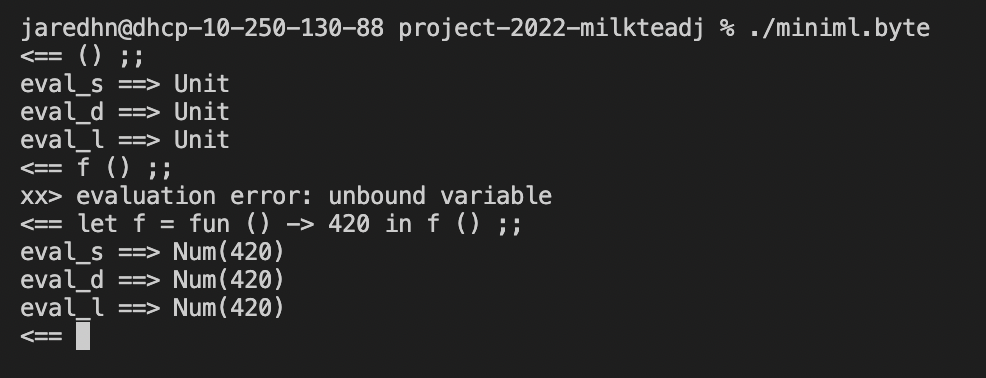
\includegraphics[width=15cm]{unit.png}\\
unit type in the MiniML interpreter
\end{center}

\pagebreak
\section{The Lexical Environment Evaluator}

My next extension is the lexical environment evaluator, eval\_l. I started off by following the instructions in the textbook and copied the code for my eval\_d into eval\_l. Luckily for me, I have already abstracted away the unop and binop operations into their own functions for all three evaluators, so it was not too much code to deal with. 

I then changed the match for Fun (function) and FunUnit (unit function) to return Env.Closure instead of Env.Val, so the state of the environment that the function evaluates using can be preserved where the function is defined. Then, based on the lexical function application rule in the textbook, I changed the return for function applications. Then, I modified the recursive definition of the lexical evaluator by using imperative reference to Unassigned type and reference reassignment, exactly as it would logically map to the direction given in stage 8 of the project in the textbook. 

Here is a demonstration of the differences between the evaluators. Lexical evaluator operations should match that of the substitution semantics in output, though it is implemented using environment semantics like that of the dynamic evaluator. A program that yields different results between dynamic and lexical scopes would be reassigning a variable after it is used in a declared function, like in the following: 

\begin{center}
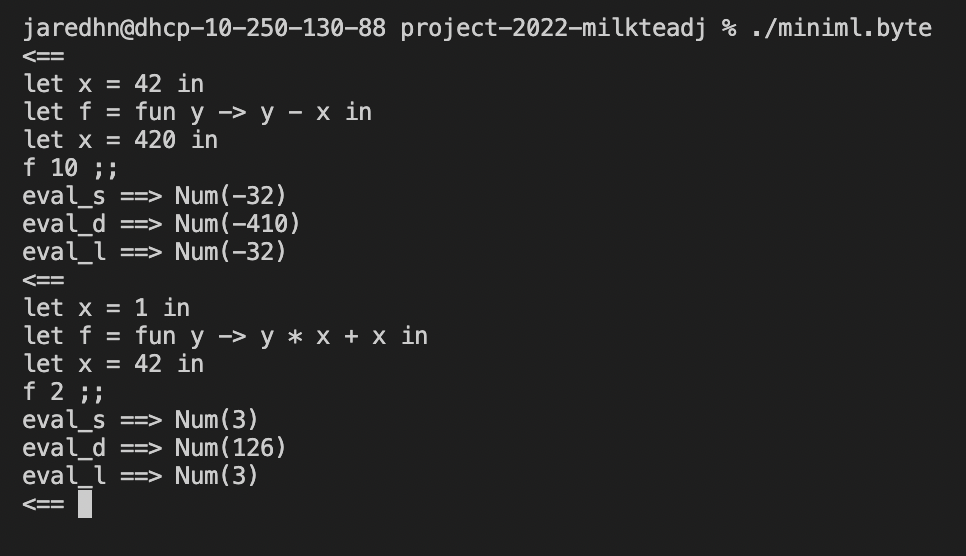
\includegraphics[width=15cm]{eval.png}\\
outputs of dynamically-scoped evaluator can differ from lexically-scoped evaluators
\end{center}



\printbibliography % If something looks strange in the bibliography, more often than not, you can modify the parameter in the .bib to fix the problem
\end{document}
